\documentclass[final]{header/fhnwreport}

%%---Main Packages-----------------------------------------------------------------------
\usepackage[english, ngerman]{babel}	%Mul­tilin­gual sup­port for LaTeX
\usepackage[T1]{fontenc}				%Stan­dard pack­age for se­lect­ing font en­cod­ings
\usepackage[utf8]{inputenc}				%Ac­cept dif­fer­ent in­put en­cod­ings
\usepackage{lmodern}                    %The newer Font-Set
\usepackage{textcomp}					%LaTeX sup­port for the Text Com­pan­ion fonts
\usepackage{graphicx} 					%En­hanced sup­port for graph­ics
\usepackage{float}						%Im­proved in­ter­face for float­ing ob­jects
\usepackage{ifdraft}                    %Let you check if the doc is in draft mode
\usepackage[toc]{glossaries}

% Glossary
\makeglossaries
\newglossaryentry{test}
{
  name=test,
  description={[...]}
}


%%---Useful Packages---------------------------------------------------------------------
\usepackage[pdftex,dvipsnames]{xcolor}  %Driver-in­de­pen­dent color ex­ten­sions for LaTeX
\usepackage{csquotes}                   %Simpler quoting with \enquote{}
\usepackage{siunitx} 					%A com­pre­hen­sive (SI) units pack­age
\usepackage{listings}					%Type­set source code list­ings us­ing LaTeX
\usepackage[bottom]{footmisc}			%A range of foot­note op­tions
\usepackage{footnote}					%Im­prove on LaTeX's foot­note han­dling
\usepackage{verbatim}					%Reim­ple­men­ta­tion of and ex­ten­sions to LaTeX ver­ba­tim
\usepackage[textsize=footnotesize]{todonotes} %Mark­ing things to do in a LaTeX doc­u­ment
\usepackage{soul}

%%---Tikz Packages-----------------------------------------------------------------------
\usepackage{standalone}
\usepackage{tikz}
\usepackage{circuitikz}
\usetikzlibrary{arrows}
\usetikzlibrary{calc}
\usetikzlibrary{intersections}

%%---Math Packages-----------------------------------------------------------------------
\usepackage{amsmath}					%AMS math­e­mat­i­cal fa­cil­i­ties for LaTeX
%\usepackage{amssymb}					%Type­set­ting symbols (AMS style)
%\usepackage{array}						%Ex­tend­ing the ar­ray and tab­u­lar en­vi­ron­ments
%\usepackage{amsthm}					%Type­set­ting the­o­rems (AMS style)

%%---Table Packages----------------------------------------------------------------------
\usepackage{tabularx}					%Tab­u­lars with ad­justable-width columns
%\usepackage{longtable}
\usepackage{multirow}					%Create tab­u­lar cells span­ning mul­ti­ple rows
\usepackage{multicol}					%In­ter­mix sin­gle and mul­ti­ple columns

%%---PDF / Figure Packages---------------------------------------------------------------
\usepackage{pdfpages}					%In­clude PDF doc­u­ments in LaTeX
\usepackage{pdflscape}					%Make land­scape pages dis­play as land­scape
\usepackage{subfig}					    %Fig­ures di­vided into sub­fig­ures

%%---Other Packages----------------------------------------------------------------------
%\usepackage{xargs}                     %De­fine com­mands with many op­tional ar­gu­ments

%%---Bibliography------------------------------------------------------------------------
\usepackage[style=ieee,urldate=comp,backend=biber]{biblatex}
\addbibresource{sections/bibliography.bib}

%%---Main Settings-----------------------------------------------------------------------
\graphicspath{{./graphics/}}			%Defines the graphicspath
%\geometry{twoside=false}				    %twoside=false disables the "bookstyle"
\setlength{\marginparwidth}{2cm}
\overfullrule=5em						%Creates a black rule if text goes over the margins => debugging

%%---User Definitions--------------------------------------------------------------------
%% Tabel-Definitions: (requires \usepackage{tabularx})
\newcolumntype{L}[1]{>{\raggedright\arraybackslash}p{#1}}    %column-width and alignment
\newcolumntype{C}[1]{>{\centering\arraybackslash}p{#1}}
\newcolumntype{R}[1]{>{\raggedleft\arraybackslash}p{#1}}

%% MONTH
\newcommand{\MONTH}{
	\ifcase\the\month
	\or January
	\or February
	\or March
	\or April
	\or May
	\or June
	\or July
	\or August
	\or September
	\or October
	\or November
	\or December
	\fi}
\urlstyle{same}
\definecolor{link}{rgb}{.02,.388,.757}
\definecolor{gray1}{gray}{0.75}
\definecolor{gray2}{gray}{0.85}
\setul{1.15pt}{.4pt}

%% Equation Parameters Description
% Source: https://tex.stackexchange.com/questions/95838/how-to-write-a-perfect-equation-parameters-description/95845#95845
\newenvironment{conditions}
{\par\vspace{\abovedisplayskip}\noindent\begin{tabular}{>{$}l<{$} @{${}={}$} l}}
	{\end{tabular}\par\vspace{\belowdisplayskip}}

%% Harpoon-Vector
\makeatletter
\newcommand{\vect}{\mathpalette{\overarrowsmall@\rightharpoonfill@}}
\def\rightharpoonfill@{\arrowfill@\relbar\relbar\rightharpoonup}
\newcommand{\overarrowsmall@}[3]{
	\vbox{
		\ialign{
			##\crcr
			#1{\smaller@style{#2}}\crcr
			\noalign{\nointerlineskip}
			$\m@th\hfil#2#3\hfil$\crcr
		}
	}
}
\def\smaller@style#1{
	\ifx#1\displaystyle\scriptstyle\else
	\ifx#1\textstyle\scriptstyle\else
	\scriptscriptstyle
	\fi
	\fi
}
\makeatother

%%---Optional Package Settings-----------------------------------------------------------
%Listings-Settings: (requires \usepackage{listings}) => Example with Matlab Code
\lstset{language=Matlab,%
    basicstyle=\footnotesize\ttfamily,
    breaklines=false,%
    morekeywords={switch, case, otherwise},
    keywordstyle=\color{Blue},%
    tabsize=2,
    %morekeywords=[2]{1}, keywordstyle=[2]{\color{black}},
    identifierstyle=\color{Black},%
    stringstyle=\color{Purple},
    commentstyle=\color{Green},%
    showstringspaces=false,%without this there will be a symbol in the places where there is a space
    numbers=left,%
    numberstyle={\tiny \color{black}},% size of the numbers
    numbersep=9pt, % this defines how far the numbers are from the text
    %emph=[1]{word1, word2,...},emphstyle=[1]\color{red}
}


\makeatletter
\newcommand{\vect}{\mathpalette{\overarrowsmall@\rightharpoonfill@}}
\def\rightharpoonfill@{\arrowfill@\relbar\relbar\rightharpoonup}
\newcommand{\overarrowsmall@}[3]{
	\vbox{
		\ialign{
			##\crcr
			#1{\smaller@style{#2}}\crcr
			\noalign{\nointerlineskip}
			$\m@th\hfil#2#3\hfil$\crcr
		}
	}
}
\def\smaller@style#1{
	\ifx#1\displaystyle\scriptstyle\else
	\ifx#1\textstyle\scriptstyle\else
	\scriptscriptstyle
	\fi
	\fi
}
\makeatother

\newenvironment{conditions}
{\par\vspace{\abovedisplayskip}\noindent\begin{tabular}{>{$}l<{$} @{${}={}$} l}}
	{\end{tabular}\par\vspace{\belowdisplayskip}}

\title{\textbf{{\Huge E 6 - Magnetic Fields}}}
\author{{\Huge Physics Laboratory Report}}
\date{{\LARGE Windisch, \the\day.\MONTH \the\year}}

\begin{document}

% Physics Laboratory Notebook
\pagenumbering{gobble}
\selectlanguage{english}
\newpage
\null
\setlength{\unitlength}{1cm}
\begin{picture}(0,0)
	\linethickness{0.025mm}
	\put(-0.85,2.2){\mbox{
\includegraphics[height=12mm]{fhnw-logo/fhnw_ht_logo_en}}}
\end{picture}
\par
\textbf{\Huge Physics Laboratory Notebook}
\vskip 1cm
\begin{LARGE}
	\setlength\tabcolsep{0pt}
	\begin{tabularx}{\textwidth}{l p{0.9cm} X}
		\textbf{Experiment Leader:} & & Dominik Müller \\
		\textbf{Assistant:} & & Simon Burkhardt \\
	\end{tabularx}
\end{LARGE}
\vskip 1.5cm
\begin{center}
	\begin{Large}
		\begin{tabularx}{\textwidth}{l|l|l|X}
			\textbf{Date} & \textbf{Experiment} & \textbf{Due Date} & \textbf{Grade} \\
			\hline\hline
			& & & \\
			11.10.2018 & C - Evaluation with Computer & 25.10.2018 & \\
			& & & \\
			\hline
			& & & \\
			25.10.2018 & E 6 - Magnetic Fields & 12.11.2018 & \\
			& & & \\
			\hline
			& & & \\
			22.11.2018 & O 9 - Interference and Diffraction & 13.12.2018 & \\
			& & & \\
			\hline
		\end{tabularx}
	\end{Large}
\end{center}
\clearpage


% Title
\selectlanguage{English}
\maketitle
\vfill
\begin{LARGE}
	\begin{tabularx}{\textwidth}{l p{0cm} X}
		\hline
		& & \\
		\textbf{Experiment Leader:} & & Dominik Müller \\
		\textbf{Assistant:} & & Simon Burkhardt \\
	\end{tabularx}
\end{LARGE}
\clearpage

% Contents
\pagenumbering{Roman}		
\selectlanguage{English}
\tableofcontents
\clearpage

% Text
\pagenumbering{arabic}
\selectlanguage{English}
\section{Theoretical Foundations}
\label{sec:Theoretical_Foundations}
In this experiment the speed of sound in various solids and liquids was determined. This section summarizes the theory and formulas necessary to understand the following experiments on ultrasound in section \ref{sec:Evaluation}.

%-------------------------------------------------------------------------------------------
\subsection{Wave Propagation}
\label{subsec:Wave_Propagation}
Wave propagation is the way in which waves travel. It can be distinguished between transverse waves and longitudinal waves. These waveforms are defined as follows:

\textbf{Transverse wave:} The displacement of the medium the wave travels through is perpendicular to the direction in which the wave propagates. Figure \ref{fig:transverse} shows a graphical representation of this sinusoidal waveform in a rope \cite{waves}.

\begin{figure}[H]
	\centering
	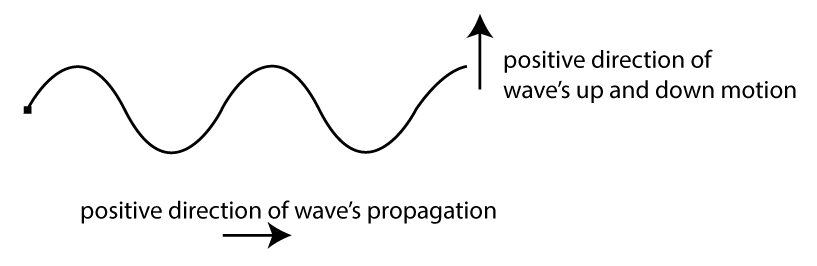
\includegraphics[scale=0.4]{transverse}
	\caption{Representation of a periodic transverse sinusoidal wave in a rope. The up and down motion of the rope is perpendicular to the direction in which the wave propagates. This leads to each particle of the rope moving up and down \cite{waves}. - partially modified}
	\label{fig:transverse}
\end{figure}

\textbf{Longitudinal wave:} The displacement of the medium the wave travels through is parallel to the direction in which the wave propagates. Sound waves in air behave like this. The air molecules oscillate back and forth and their energy is propagated in the same direction as their motion. Figure \ref{fig:longitudinal} shows a graphical representation of this waveform in a mechanical spring \cite{waves}.

\begin{figure}[H]
	\centering
	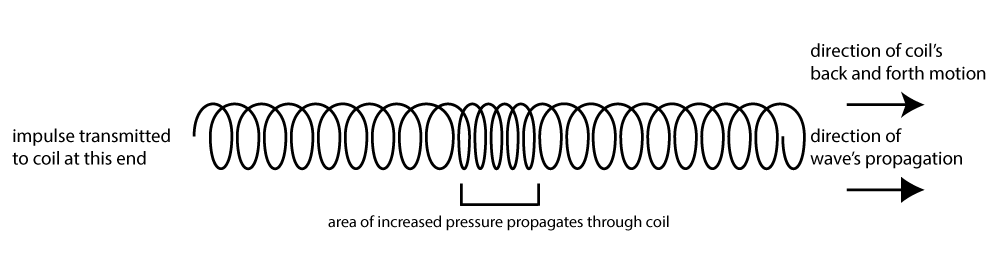
\includegraphics[scale=0.45]{longitudinal}
	\caption{Representation of a longitudinal wave in a mechanical spring. The elastic deflection (compression and extension) of the spring is parallel to the direction in which the wave propagates. This produces areas of increased and decreased pressure \cite{waves}.}
	\label{fig:longitudinal}
\end{figure}

\newpage
%-------------------------------------------------------------------------------------------
\subsection{Reflection and Refraction}
\label{subsec:Reflection_and_Refraction}
Similar to optics, reflection and refraction also occur when sound waves hit the boundary between two different media. Contrary to optics, the refraction index is not the important quantity. The phase velocity leads to refraction and the impedance leads to reflection. It can be distinguished between a vertical and an oblique angle of incidence. The following two sections explain this in more detail \cite{ultrasound}.

%-------------------------------------------------------------------------------------------
\subsubsection{Vertical Angle of Incidence}
\label{subsubsec:Vertical_Angle_of_Incidence}
A sound wave with the pressure $\hat{p}_e$ and velocity $v_e$ that travels trough a medium with the impedance $Z_1$ hits a boundary between two media with a vertical angle of incidence. This results in a different ratio between the pressure $\hat{p}_t$ and velocity $v_t$ in the medium with the impedance $Z_2$. At the same time the pressure and the velocity have to be equal at the boundary between the two media. This leads to a third reflected partial wave. Figure \ref{fig:vertical_angle_of_incidence} shows the just described phenomenon \cite{ultrasound}.

\begin{figure}[H]
	\centering
	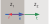
\includegraphics[scale=1.5]{vertical_angle_of_incidence}
	\caption{Representation of a sound wave $e$ in blue that hits a boundary between the two media with the impedances $Z_1$ and $Z_2$. The transmitted wave $t$ is shown in green and the reflected partial wave $r$ is shown in red \cite{ultrasound}. - partially modified}
	\label{fig:vertical_angle_of_incidence}
\end{figure}

The calculation of the amplitude reflection coefficient $r$ is shown in equation \ref{eq:vertical_reflection} and the amplitude transmission coefficient $t$ is shown in equation \ref{eq:vertical_transmission}. They can be derived by utilizing the continuity conditions that are valid at the interface between the two media \cite{ultrasound}.

\begin{equation}
r = \dfrac{\hat{p}_r}{\hat{p}_e} = \dfrac{Z_2-Z_1}{Z_2+Z_1}
\label{eq:vertical_reflection}
\end{equation}
\begin{equation}
t = \dfrac{\hat{p}_t}{\hat{p}_e} = \dfrac{2 Z_2}{Z_2+Z_1}
\label{eq:vertical_transmission}
\end{equation}
where:
\begin{multicols}{2}
\begin{conditions}
	r & reflection coefficient \\
	t & transmission coefficient \\
	Z_1 \text{, } Z_2 & medium impedance
\end{conditions}
\begin{conditions}
	\hat{p}_r & reflected pressure \\
	\hat{p}_t & transmitted pressure \\
	\hat{p}_e & pressure amplitude
\end{conditions}
\end{multicols}

If $Z_2$ is smaller than $Z_1$ the reflection coefficient turns out negative which means the reflected wave is phase-shifted by 180\textdegree\ \cite{ultrasound}.
\newpage
%-------------------------------------------------------------------------------------------
\subsubsection{Oblique Angle of Incidence}
\label{subsubsec:Oblique_Angle_of_Incidence}
The reflection and transmission coefficients of a sound wave $e$ that hits an interface between two media with an oblique angle $\alpha$ depend on this angle of incidence. Furthermore, the transmitted wave will be refracted. If the medium $Z_2$ happens to be a solid, a transversal and a longitudinal wave will form. Figure \ref{fig:oblique_angle_of_incidence} shows this phenomenon which is called \flqq mode conversion\frqq\ \cite{ultrasound}.

\begin{figure}[H]
	\centering
	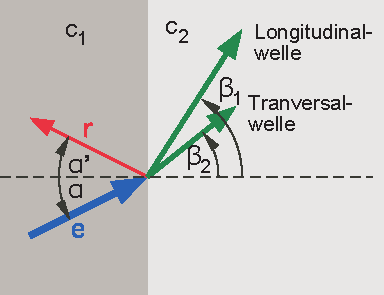
\includegraphics[scale=1.5]{oblique_angle_of_incidence}
	\caption{Representation of a sound wave $e$ shown in blue that hits an interface between the two media $Z_1$ and $Z_2$ with an oblique angle of incidence. The reflected wave $r$ is shown in red and the refracted transverse and longitudinal waves are shown in green \cite{ultrasound}.}
	\label{fig:oblique_angle_of_incidence}
\end{figure}

To calculate the angle of reflection shown in equation \ref{eq:oblique_angle_of_incidence} and the refraction shown in equation \ref{eq:oblique_refraction}, the same known laws from optics apply. Equation \ref{eq:oblique_refraction} allows the use of the transversal or longitudinal sound velocity for the variable $c_2$ depending on the desired result \cite{ultrasound}.

\begin{equation}
\alpha = \alpha^\prime
\label{eq:oblique_angle_of_incidence}
\end{equation}
\begin{equation}
\dfrac{\sin{(\alpha)}}{\sin{(\beta)}} = \dfrac{c_1}{c_2}
\label{eq:oblique_refraction}
\end{equation}
where:
\begin{multicols}{2}
\begin{conditions}
	\alpha & angle of incidence \\
	\beta & angle of refraction
\end{conditions}
\begin{conditions}
	\alpha^\prime & angle of reflection \\
	c_1 \text{, } c_2 & sound velocity in the medium
\end{conditions}
\end{multicols}


%-------------------------------------------------------------------------------------------
\subsection{Total Internal Reflection}
\label{subsec:Total_Internal_Reflection}
Total internal reflection can take place at the interface between two media. This happens when the following equation is valid:

\[
\sin{(\alpha_\text{crit})} = \dfrac{c_1}{c_2}
\]

This is a variation of the above shown equation \ref{eq:oblique_refraction}. Thus, the angle of refraction $\beta$ has to be 90\textdegree\ for the equation to be valid. For $\alpha \geq \alpha_\text{crit}$ the wave is totally reflected \cite{ultrasound}.

%-------------------------------------------------------------------------------------------
\subsection{Absorption}
\label{subsec:Absorption}
Sound waves are attenuated when they propagate in a medium due to absorption and scattering. Absorption usually converts a part of the ultrasound wave into heat. Scattering leads a particle that has been excited by the incoming wave to emit a wave in all direction itself. Equation \ref{eq:absorption} shows the exponential attenuation for monochromatic radiation. The \textbf{higher the frequency}, the \textbf{stronger the absorption} and scattering \cite{ultrasound}.

\begin{equation}
\hat{p}(x) = \hat{p}_0 \cdot e^{-\mu x}
\label{eq:absorption}
\end{equation}
where:
\begin{multicols}{2}
\begin{conditions}
	\hat{p}(x) & attenuated amplitude \\
	\mu & attenuation coefficient in m$^{-1}$
\end{conditions}
\begin{conditions}
	\hat{p}_0 & initial amplitude \\
	x & distance in m
\end{conditions}
\end{multicols}

%-------------------------------------------------------------------------------------------
\subsection{Ultrasound Generation}
\label{subsec:Ultrasound_Generation}
Ultrasound can be generated and received by using a ultrasonic transducer. In this experiment the piezoelectric effect is used in the ultrasonic transducer. Certain crystals expand proportional to the applied voltage. Contrary to this, the piezoelectric transducer induces a voltage when deformed. Thus, it can be used as a transmitter or receiver \cite{ultrasound}.

\begin{figure}[H]
	\centering
	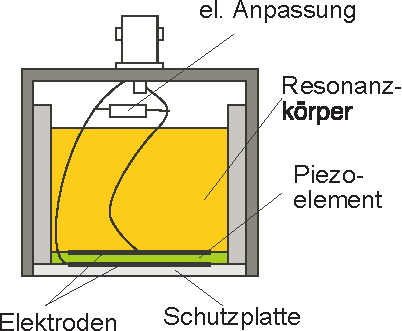
\includegraphics[scale=1.5]{ultrasound_generation}
	\caption{Graphical representation of a piezoelectric transducer. The active part is the thin piezo disk at the bottom of the transducer. The mechanical dimensions determine the resonance frequency of the oscillation. The transducer is impedance matched to the amplifier \cite{ultrasound}.}
	\label{fig:ultrasound_generation}
\end{figure}

\newpage
%-------------------------------------------------------------------------------------------
\subsection{Ultrasound Measurement}
\label{subsec:Ultrasound_Measurement}
There are two common ways to measure ultrasound, the A-Scan and the B-Scan. This experiment uses the A-Scan as measurement method and therefore only this one will be explained.

The A-Scan is a one-dimensional procedure where short ultrasound impulses ($f > 20 \text{kHz}$) are transmitted. These are partially reflected on the interfaces between media and are received again by the transmitter. From the time difference between the sent impulse and the received echo and a known distance, the sound velocity of a medium can be determined. Equation \ref{eq:sound_velocity} shows this relationship \cite{ultrasound}.

\begin{equation}
c_m = \dfrac{2x}{\Delta t}
\label{eq:sound_velocity}
\end{equation}
where:
\begin{multicols}{2}
	\begin{conditions}
		c_m & sound velocity of a medium in $\,^{\text{m}}\!/_{\text{s}}$ \\
		\Delta t & time difference in s
	\end{conditions}
	\begin{conditions}
		x & distance to interface in m
	\end{conditions}
\end{multicols}

This technique is often used to check the integrity of materials. If the part has defects such as cracks or inclusions of different substances, there are detectable echoes. Furthermore, the wall thickness of work pieces can be determined by this method \cite{ultrasound}.

\section{Conducting the Experiments}
\label{sec:Conducting_the_Experiments}
This section describes the experimental arrangement with the device list and all the measurement objects. Furthermore, it contains information about the measuring process. All measurements were conducted at 21 \textdegree C room temperature.

\subsection{Measurements}
\label{subsec:Measurements}
In this experiment, the following measurements were conducted:

\begin{enumerate}
	\item Wave length of sound waves in air, distilled water and aluminium for 1 kHz, 1 MHz and 5 MHz calculated from literature data
	\item Ultrasound velocity (longitudinal, reflection) for 1 MHz and 5 MHz in
	\begin{itemize}
		\item PMMA object
		\item Aluminium cylinder
		\item Copper cylinder
		\item Brass cylinder
	\end{itemize}
	\item Attenuation coefficient of PMMA for 1 MHz and 5 MHz
	\item Ultrasound velocity (longitudinal, reflection) for 5 MHz in
	\begin{itemize}
		\item Water at 20 \textdegree C
		\item Water at 50 \textdegree C
		\item Saltwater at 40 \textdegree C
	\end{itemize}
	\item Ultrasound velocity (transversal, reflection) for 1 MHz in PMMA
\end{enumerate}

\subsection{Experimental Arrangement}
\label{subsec:experimental_arrangement}
The experiment was arranged as shown below in figure \ref{fig:experimental_arrangement}:
\begin{figure}[H]
	\centering
	\includegraphics[scale=0.11]{experimental_arrangement}
	\caption{Annotated picture of the experimental arrangement for measurement no. 5: Ultrasound velocity (transverse, reflection) for 1 MHz in PMMA. For this measurement a special kind of ultrasound gel had to be used, as the transversal sound velocity was measured.}
	\label{fig:experimental_arrangement}
\end{figure}

\newpage
To measure the ultrasound velocity in water, a water bath and a reflector were used. This is shown in figure \ref{fig:experimental_arrangement_water_bath}:

\begin{figure}[H]
	\centering
	\includegraphics[scale=0.11]{experimental_arrangement_water_bath}
	\caption{Annotated picture of the experimental arrangement for measurement no. 4: Ultrasound velocity (longitudinal, reflection) for 5 MHz in saltwater at 40 \textdegree C. For this measurement the saltwater had to be heated up to the desired temperature with a heater and a magnetic stirrer.}
	\label{fig:experimental_arrangement_water_bath}
\end{figure}

The following equipment was used:

\begin{table}[H]
	\centering
	\renewcommand{\arraystretch}{1.2}
	\begin{tabular}{l l l}
		\hline
		\textbf{Device} & \textbf{Designation} & \textbf{Uncertainty} \\
		\hline
		Ultrasonic pulser / receiver unit & Olympus 5077PR (P-M5-025) & N/A \\
		Transducer 1 MHz (transverse) & Parametrics NDT V153 & N/A \\
		Transducer 1 MHz & Parametrics NDT V102 (892817) & N/A \\
		Transducer 5 MHz & Parametrics NDT V107 (900322) & N/A \\
		Oscilloscope & LeCroy WaveRunner 64MXi-A & $\pm0.05$ V / $\pm0.1\ \si{\mu s}$ \\
		Thermometer & Keithley 132C TRMS Multimeter & $\pm1$ \textdegree C \\
		Calliper & Mitutoyo CD-15PPX (13021983) & $\pm0.01$ mm \\
		Heater & IKA RCT basic (P-P8-052) & N/A \\
		Scale & OHAUS Scout Pro & N/A \\ \hline
	\end{tabular}
	\caption{List of the used equipment and measurement devices including test equipment number if available. Furthermore, the uncertainty is stated for all of the measurement devices (not for the regular equipment).}
	\label{tab:equipment}
\end{table}

\newpage
\subsection{Measurement Objects}
\label{subsec:measurement_objects}
The measuring objects are a range of different materials (PMMA, aluminium, copper, brass, water). The following figure \ref{fig:measurement_objects} shows the PMMA object, and the metal cylinders:

\begin{figure}[H]
	\centering
	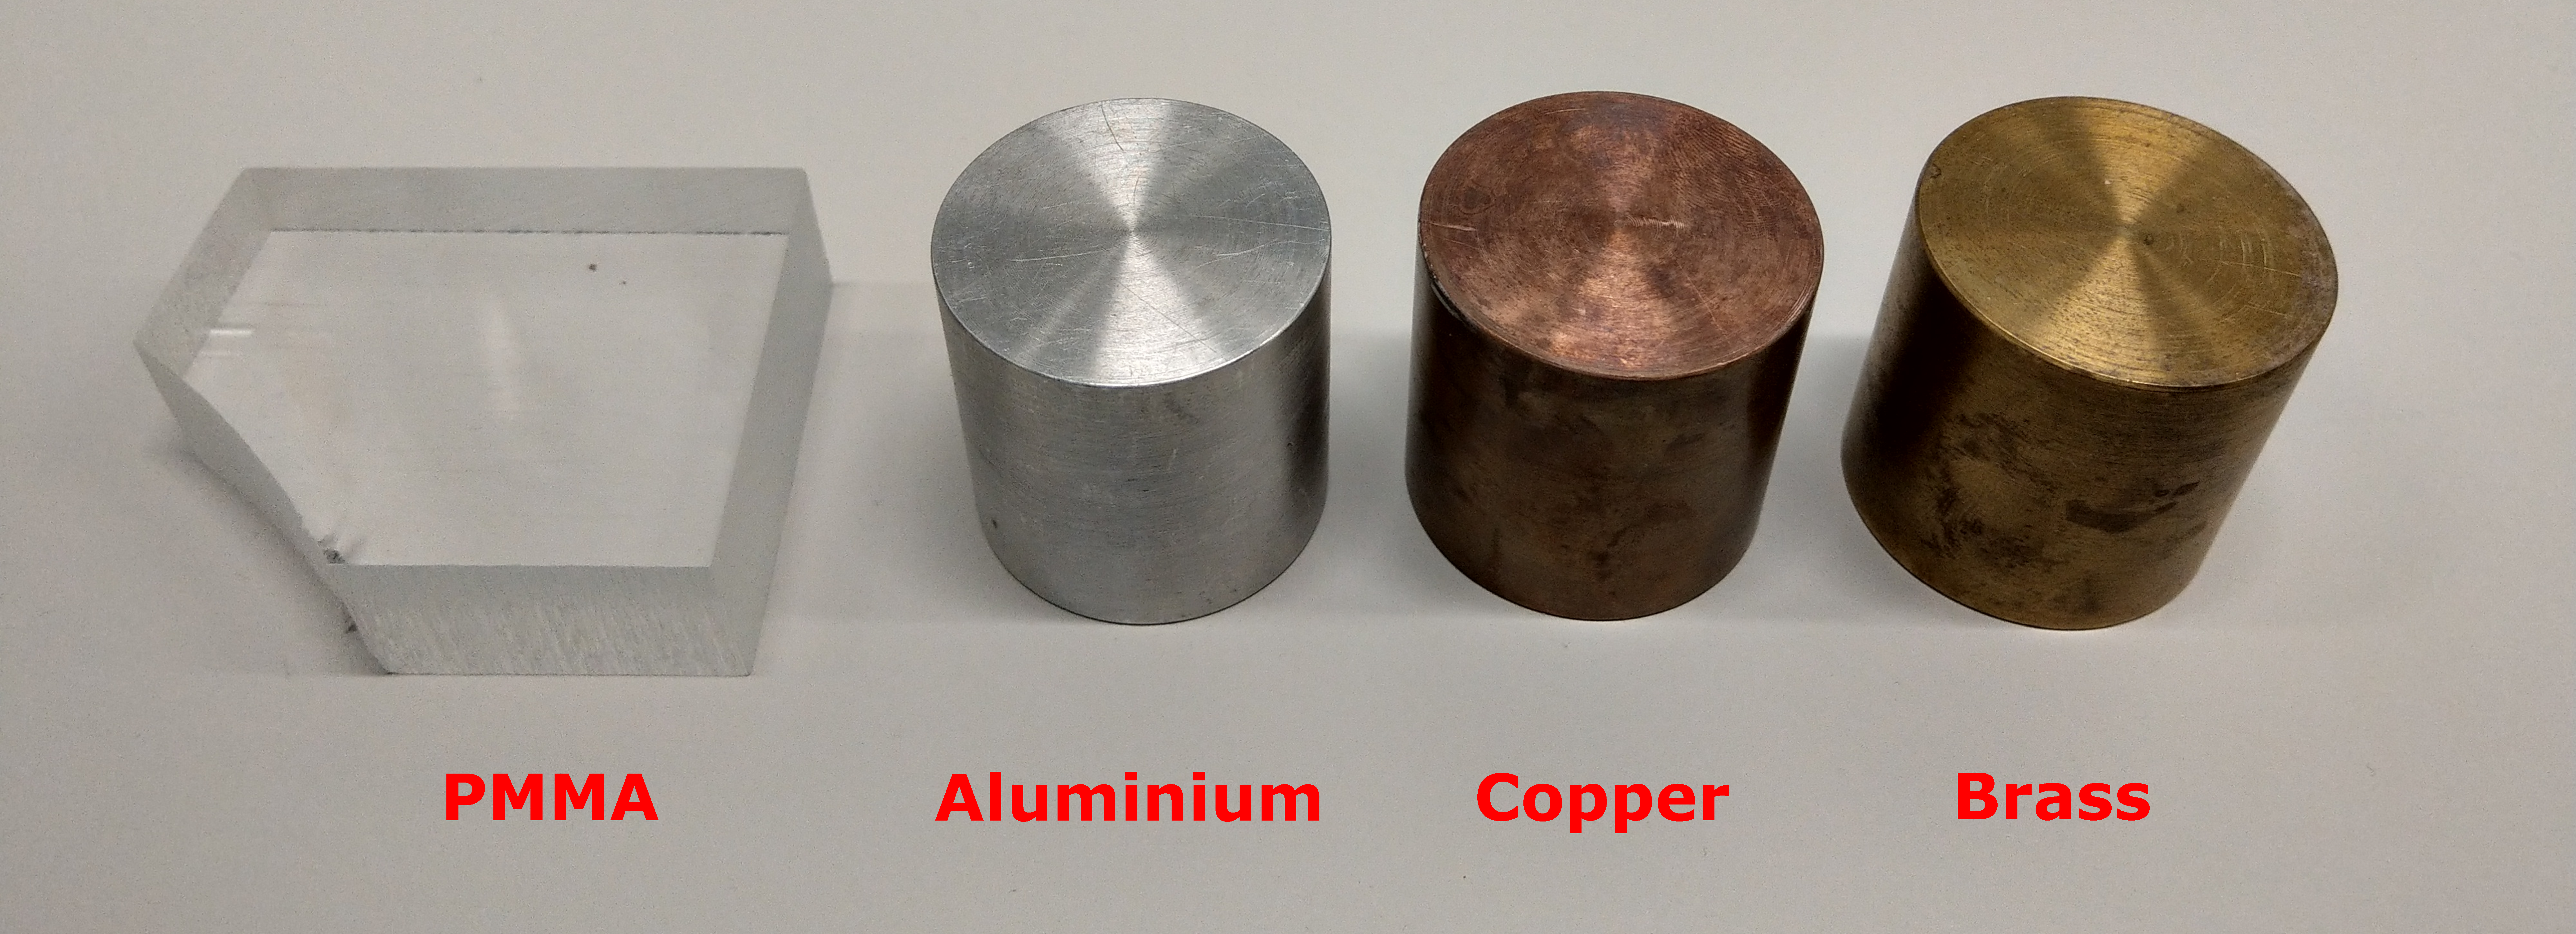
\includegraphics[scale=0.11]{measurement_objects}
	\caption{Annotated picture of the measurement objects used in measurements no. 2, 3 and 5. A PMMA object and three different metals (aluminium, copper and brass) were used.}
	\label{fig:measurement_objects}
\end{figure}

The different objects and their sound path distances are listed in the table \ref{tab:sound_path_distance} below.

\begin{table}[H]
	\centering
	\renewcommand{\arraystretch}{1.2}
	\begin{tabular}{r|l}
		 & \textbf{Sound Path Distance $x$} \\
		\hline
		\textbf{PMMA object} & $(20.40 \pm 0.01)\ \si{mm}$ \\
		\textbf{Aluminium cylinder} & $(40.03 \pm 0.01)\ \si{mm}$ \\
		\textbf{Copper cylinder} & $(40.05 \pm 0.01)\ \si{mm}$ \\
		\textbf{Brass cylinder} & $(40.06 \pm 0.01)\ \si{mm}$ \\
		\textbf{Water bath} & 0 mm up to $(180 \pm 0.1)\ \si{mm}$ \\ \hline
	\end{tabular}
	\caption{Specifications of the measured objects}
	\label{tab:sound_path_distance}
\end{table}

\subsection{Measuring Procedure}
\label{subsec:measuring_procedure}
The oscilloscope is connected to the ultrasonic pulser / receiver unit and shows the attenuated echoes received by the piezoelectric transducer. The time of flight (the duration it takes the sound wave to travel through the medium and return back to the transducer) is measured with the vertical cursors. Similarly, the amplitude is measured with the horizontal cursors. Figure \ref{fig:measuring_procedure} shows the waveform measured on the oscilloscope with a 5 MHz transducer in PMMA.

\begin{figure}[H]
	\centering
	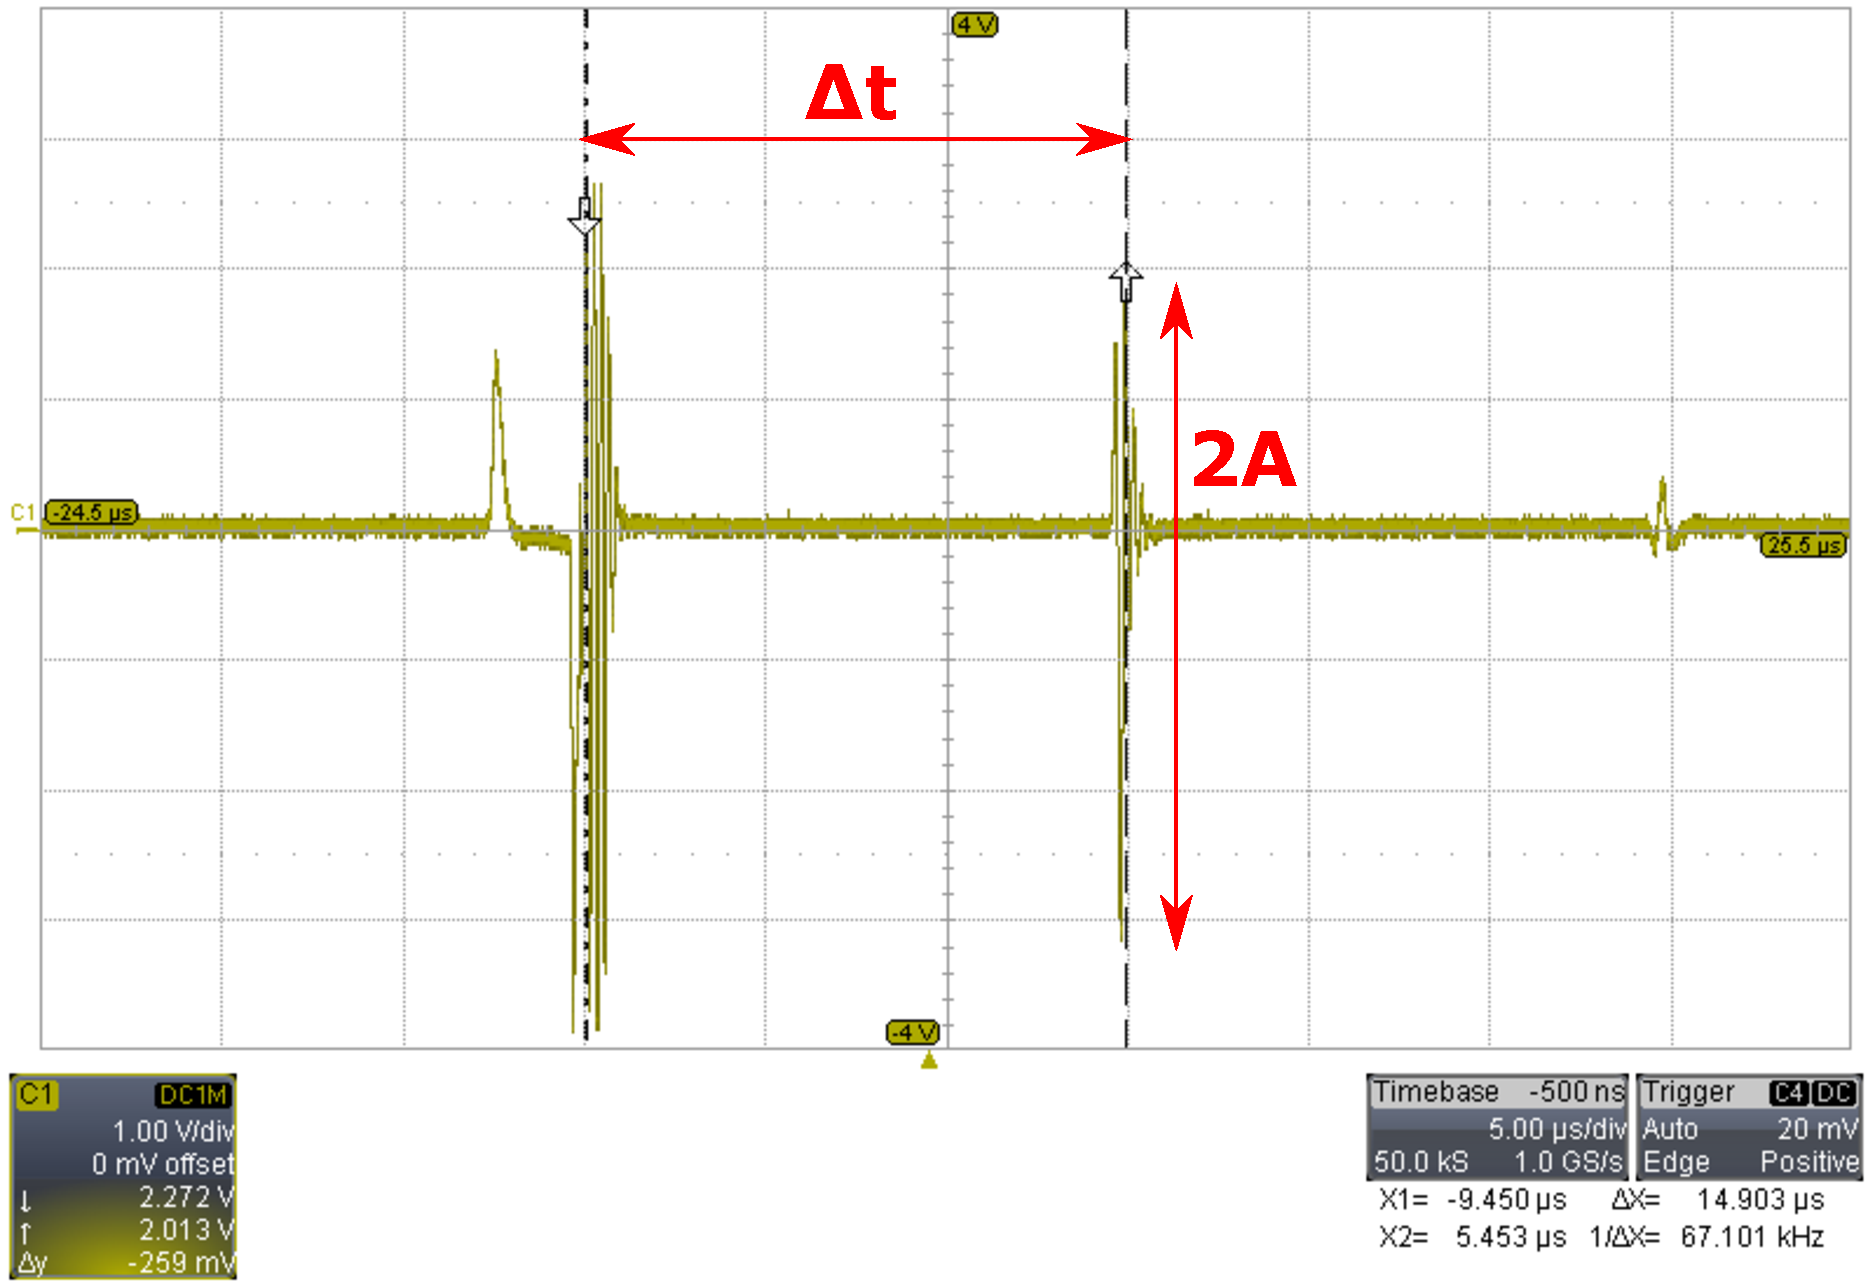
\includegraphics[scale=0.5]{measuring_procedure}
	\caption{Annotated picture of the waveform shown on the oscilloscope. The time of flight $\Delta t$ and the amplitude $A$ are marked in red. The peaks are the echoes that occur when the wave is totally reflected. The initial small peak is likely a reflection on the bottom plate of the piezoelectric transducer.}
	\label{fig:measuring_procedure}
\end{figure}

\section{Evaluation}
\label{sec:Evaluation}
This section contains the evaluation and the graphical representation of the measurements.

\subsection{Slit Apertures}
\label{subsec:Slit}
The angle $\varphi$ was measured indirectly by measuring the distance from the slit aperture to the projection surface and the position of the maxima. All measured values are listed in appendix \ref{sec:Measurements} and the MATLAB code which calculates the angle using equation \ref{eq:angle} is listed in appendix \ref{sec:MATLAB_Angle_Calculation}.
\begin{figure}[H]
	\centering
	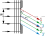
\includegraphics[scale=1]{slit}
	\caption{Slit Apertures}
	\label{fig:Slit}
\end{figure}
Figure \ref{fig:Slit} shows the indirectly measured angles $\varphi$ (see table \ref{tab:Slit_Measurements}) at several different orders $m$ and the according linear fit. The black dots were measured with the 40 $\mu$m slit aperture and the red squares were measured with the 100 $\mu$m slit aperture. To create the linear fit, equation \ref{eq:slit_maxima} was used for both slit apertures. The wavelength $\lambda$ was set to its according value (633 nm) and marked as constant.

The parameters of the linear fitted curve are listed in the following table:
\begin{table}[H]
	\centering
	\renewcommand{\arraystretch}{1.3}
	\begin{tabular}{r|c c}
		& \textbf{Slit 40 $\mu$m} & \textbf{Slit 100 $\mu$m} \\
		\hline\hline
		\textbf{Width} $w$ & $(39.41\pm0.10)$ $\mu$m & $(101.26\pm0.14)$ $\mu$m \\		
		\textbf{Wavelength} $\lambda$ & \multicolumn{2}{c}{633 nm (constant)}
	\end{tabular}
	\caption{Fit Parameters (Slit Apertures)}
	\label{tab:Slit}
\end{table}
\newpage
\subsection{Anti-Slit Apertures}
\label{subsec:Anti-Slit}
Once again the angle $\varphi$ was measured indirectly by measuring the distance from the anti-slit aperture to the projection surface and the position of the maxima. The measured values are listed in appendix \ref{sec:Measurements} and the MATLAB code used to calculate the angle is again listed in appendix \ref{sec:MATLAB_Angle_Calculation}.
\begin{figure}[H]
	\centering
	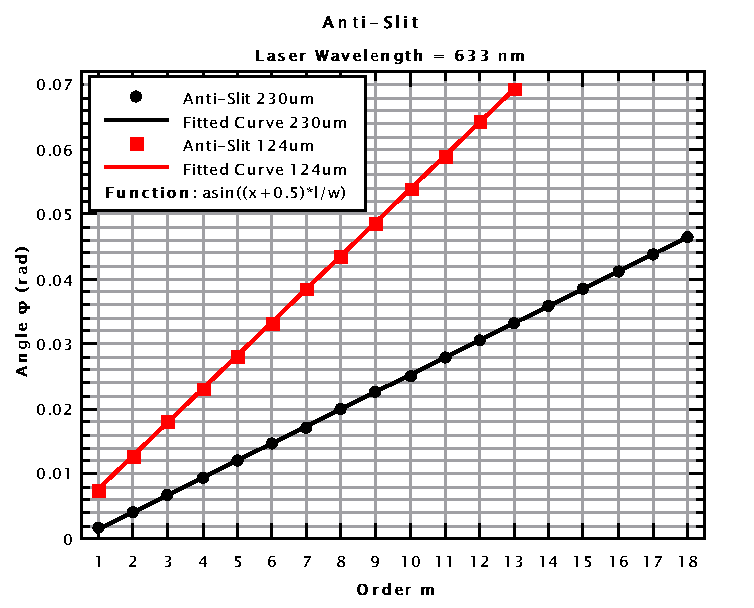
\includegraphics[scale=1]{anti-slit}
	\caption{Anti-Slit Apertures}
	\label{fig:Anti-Slit}
\end{figure}
Figure \ref{fig:Anti-Slit} shows the indirectly measured angles $\varphi$ (see table \ref{tab:Anti-Slit_Measurements}) at several different orders $m$ and the according linear fit. The black dots were measured with the 230 $\mu$m anti-slit aperture and the red squares were measured with the 124 $\mu$m anti-slit aperture. To create the linear fit, equation \ref{eq:slit_maxima} was used for both anti-slit apertures. The wavelength $\lambda$ was set to its according value (633 nm) and marked as constant.

The parameters of the linear fitted curve are listed in the following table:
\begin{table}[H]
	\centering
	\renewcommand{\arraystretch}{1.3}
	\begin{tabular}{r|c c}
		& \textbf{Anti-Slit 230 $\mu$m} & \textbf{Anti-Slit 124 $\mu$m} \\
		\hline\hline
		\textbf{Width} $w$ & $(239.10\pm0.34)$ $\mu$m & $(123.39\pm0.08)$ $\mu$m \\		
		\textbf{Wavelength} $\lambda$ & \multicolumn{2}{c}{633 nm (constant)}
	\end{tabular}
	\caption{Fit Parameters (Anti-Slit Apertures)}
	\label{tab:Anti-Slit}
\end{table}
\newpage
\subsection{Circular Apertures}
\label{subsec:Circular_Apertures}
The angle $\varphi$ was again measured indirectly by measuring the distance from the circular aperture to the projection surface. However, this time the positions of the minima were measured instead of the maxima. This is due to the lack of an easy equation to relate the maxima created by a circular aperture. The measured values are listed in appendix \ref{sec:Measurements} and the MATLAB code used to calculate the angle is listed in appendix \ref{sec:MATLAB_Angle_Calculation}.
\begin{figure}[H]
	\centering
	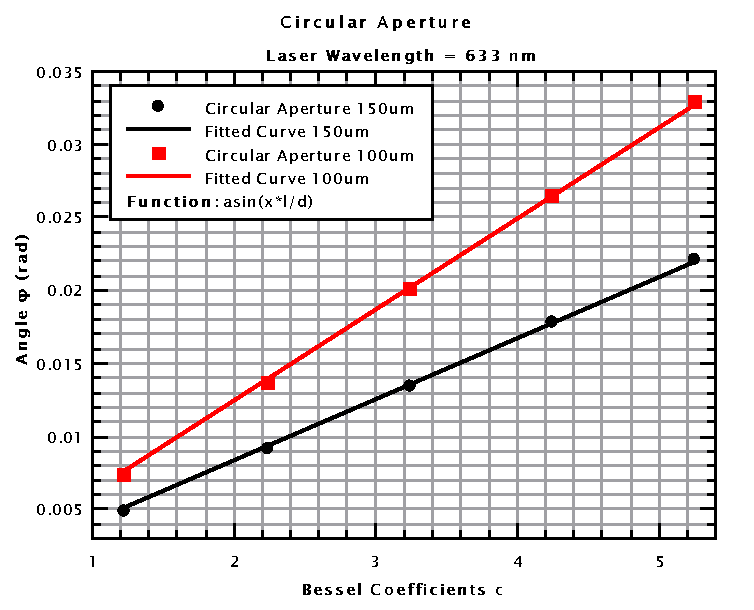
\includegraphics[scale=1]{circular_aperture}
	\caption{Circular Apertures}
	\label{fig:Circular_Apertures}
\end{figure}
Figure \ref{fig:Circular_Apertures} shows the indirectly measured angles $\varphi$ of the minima (see table \ref{tab:Circular_Apertures_Measurements}) at the first five Bessel coefficients $c_k$ (see equation \ref{eq:coeffs}) and the according linear fit. The black dots were measured with the 150 $\mu$m circular aperture and the red squares were measured with the 100 $\mu$m circular aperture. To create the linear fit, equation \ref{eq:circular_aperture} was used for both circular apertures. The wavelength $\lambda$ was set to its according value (633 nm) and marked as constant.

The parameters of the linear fitted curve are listed in the following table:
\begin{table}[H]
	\centering
	\renewcommand{\arraystretch}{1.3}
	\begin{tabular}{r|c c}
		& \textbf{Diameter 150 $\mu$m} & \textbf{Diameter 100 $\mu$m} \\
		\hline\hline
		\textbf{Diameter} $d$ & $(151.39\pm0.83)$ $\mu$m & $(101.62\pm0.55)$ $\mu$m \\		
		\textbf{Wavelength} $\lambda$ & \multicolumn{2}{c}{633 nm (constant)}
	\end{tabular}
	\caption{Fit Parameters (Circular Apertures)}
	\label{tab:Circular_Apertures}
\end{table}
\newpage
\subsection{Cross-Grid Apertures}
\label{subsec:Cross-Grid}
The angle $\varphi$ was measured indirectly by measuring the distance from the cross-grid aperture to the projection surface and the position of the maxima. All measured values are listed in appendix \ref{sec:Measurements} and the MATLAB code which calculates the angle using equation \ref{eq:angle} is listed in appendix \ref{sec:MATLAB_Angle_Calculation}.
\begin{figure}[H]
	\centering
	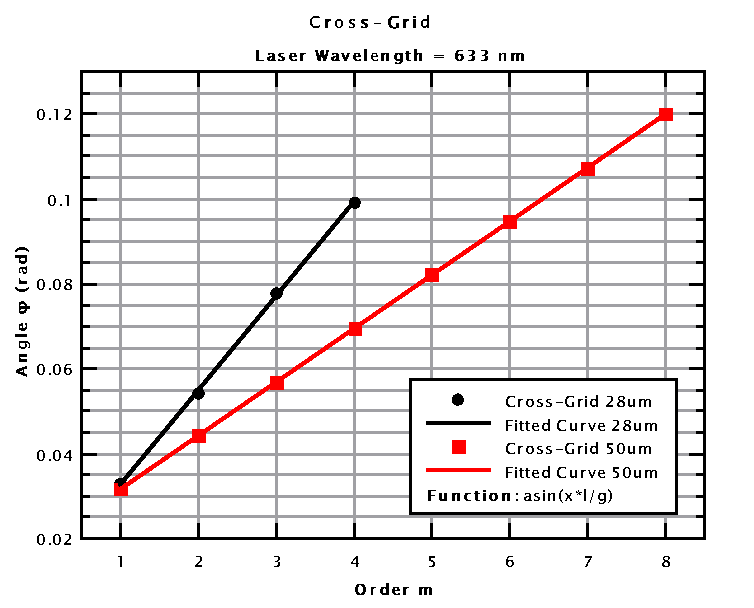
\includegraphics[scale=1]{cross-grid}
	\caption{Cross-Grid Apertures}
	\label{fig:Cross-Grid}
\end{figure}
Figure \ref{fig:Cross-Grid} shows the indirectly measured angles $\varphi$ (see table \ref{tab:Cross-Grid_Measurements}) at several orders $m$ and the according linear fit. The black dots were measured with a cross-grid that has a grid constant of 28 $\mu$m and the red squares were measured with a cross-grid that has a grid constant of 50 $\mu$m. To create the linear fit, equation \ref{eq:cross-grid} was used for both cross-grid apertures. The wavelength $\lambda$ was set to its according value (633 nm) and marked as constant.

The parameters of the linear fitted curve are listed in the following table:
\begin{table}[H]
	\centering
	\renewcommand{\arraystretch}{1.3}
	\begin{tabular}{r|c c}
		& \textbf{Cross-Grid 28 $\mu$m} & \textbf{Cross-Grid 50 $\mu$m} \\
		\hline\hline
		\textbf{Grid Constant} $g$ & $(28.53\pm0.44)$ $\mu$m & $(50.22\pm0.06)$ $\mu$m \\		
		\textbf{Wavelength} $\lambda$ & \multicolumn{2}{c}{633 nm (constant)}
	\end{tabular}
	\caption{Fit Parameters (Cross-Grid Apertures)}
	\label{tab:Cross-Grid}
\end{table}

\section{Error Calculation}
\label{sec:Error_Calculation}
This section contains the error calculation of the measured values. The error calculation is done for the fitted vacuum permeability $\mu_0$ (see sections \ref{subsubsec:Short_Cylindrical_Coil} to \ref{subsubsec:Long_Cylindrical_Coil_Field}).

\subsection{Uncertainties}
\label{subsec:Uncertainties}
All conducted measurements in this experiment have uncertainties. The uncertainty of the gaussmeter and the Hall sensor is really small (only 0.3 \%) compared to the other uncertainties. This means that it could be neglected. In this exercise it is considered nevertheless. The systematic uncertainties are shown in table \ref{tab:measurement_devices_and_sensors} and table \ref{tab:Specifications_Cylindrical_Coils} (the uncertainty of the radius $R$ is only half of the uncertainty of the diameter $d$).

\subsection{Calculating the Uncertainty of $\mu_0$}
\label{subsec:Calculating_the_Uncertainty}
To derive the total uncertainty of the vacuum permeability $\mu_0$ the following equations are used. The statistical uncertainty is obtained from the fits (from QtiPlot).
\begin{equation}
s_{\mu_{0,\ TOT}}=\sqrt{s_{\mu_{0,\ SYST}}^2+s_{\mu_{0,\ STAT}}^2}
\label{eq:total_uncert}
\end{equation}
with:
\begin{equation}
s_{\mu_{0,\ SYST}}=\sqrt{\left(\frac{\partial \mu_0}{\partial B_0}\Biggr|_{\mu_0}\cdot s_{B_0}\right)^2 + \left(\frac{\partial \mu_0}{\partial I}\Biggr|_{\mu_0}\cdot s_{I}\right)^2 + \left(\frac{\partial \mu_0}{\partial l}\Biggr|_{\mu_0}\cdot s_{l}\right)^2 + \left(\frac{\partial \mu_0}{\partial R}\Biggr|_{\mu_0}\cdot s_{R}\right)^2}
\label{eq:error_propagation}
\end{equation}

and with:

\[
\frac{\partial \mu_0}{\partial B_0}\Biggr|_{\mu_0}=\frac{l}{NI}\cdot\sqrt{1+(\,^{2R}\!/_{l})^2} \qquad , \qquad \frac{\partial \mu_0}{\partial I}\Biggr|_{\mu_0}=-\frac{B_0l}{NI^2}\cdot\sqrt{1+(\,^{2R}\!/_{l})^2}
\]

\[
\frac{\partial \mu_0}{\partial l}\Biggr|_{\mu_0}=\frac{B_0}{NI}\cdot\frac{1}{\sqrt{1+(\,^{2R}\!/_{l})^2}} \qquad , \qquad \frac{\partial \mu_0}{\partial R}\Biggr|_{\mu_0}=\frac{4B_0R}{lNI}\cdot\frac{1}{\sqrt{1+(\,^{2R}\!/_{l})^2}}
\]

where:
\begin{conditions}
	s_{\mu_{0,\ TOT}} & total uncertainty of $\mu_0$ \\
	s_{\mu_{0,\ SYST}} & systematical uncertainty of $\mu_0$ \\
	s_{\mu_{0,\ STAT}} & statistical uncertainty of $\mu_0$ (obtained from a fit) \\
	B_0 & magnetic field in the center \\
	\mu_0 & vacuum permeability \\
	N & number of turns \\
	I & current \\
	l & length \\
	R & radius
\end{conditions}

\subsection{Calculated Uncertainties $\mu_0$}
\label{subsec:Calculated_Uncertainties}
The systematic uncertainty was calculated using equation \ref{eq:error_propagation} and the statistical uncertainty was obtained from the fits (see sections \ref{subsubsec:Short_Cylindrical_Coil} to \ref{subsubsec:Long_Cylindrical_Coil_Field}). The total uncertainty was calculated by using equation \ref{eq:total_uncert}.
\begin{table}[H]
	\centering
	\renewcommand{\arraystretch}{1.3}
	\begin{tabular}{r||c|c|c}
		 & \textbf{Systematic} $(\,^\text{Vs}\!/_\text{Am})$ & \textbf{Statistical} $(\,^\text{Vs}\!/_\text{Am})$ & \textbf{Total} $(\,^\text{Vs}\!/_\text{Am})$ \\
		\hline\hline
		\textbf{Short Center} (sec. \ref{subsubsec:Short_Cylindrical_Coil}) & $1.92167\cdot10^{-8}$ & $1.87622\cdot10^{-10}$ & $1.92176\cdot10^{-8}$ \\
		\textbf{Short Field} (sec. \ref{subsubsec:Short_Cylindrical_Coil_Field}) & $1.92288\cdot10^{-8}$ & $6.34659\cdot10^{-10}$ & $1.92393\cdot10^{-8}$ \\
		\textbf{Long Center} (sec. \ref{subsubsec:Long_Cylindrical_Coil}) & $1.48213\cdot10^{-8}$ & $1.57922\cdot10^{-10}$ & $1.48221\cdot10^{-8}$ \\
		\textbf{Long Field} (sec. \ref{subsubsec:Long_Cylindrical_Coil_Field}) & $1.47958\cdot10^{-8}$ & $3.64561\cdot10^{-10}$ & $1.48003\cdot10^{-8}$ \\
	\end{tabular}
	\caption{Calculated Uncertainties}
	\label{tab:Calculated_Uncertainties}
\end{table}

To calculate the systematic uncertainty of the short coil (center value) the measurement point where the current $I=0.42$\ A was used (see table \ref{tab:Short_Cylindrical_Coil_Measurements_Central_Value}).

To calculate the systematic uncertainty of the short coil (field pattern) the measurement point which is closest to the center was used. The position of this point is $z=-0.003$\ m (see table \ref{tab:Short_Cylindrical_Coil_Measurements_Field_Pattern}).

To calculate the systematic uncertainty of the long coil (center value) the measurement point where the current $I=0.521$\ A was used (see table \ref{tab:Long_Cylindrical_Coil_Measurements_Central_Value}).

To calculate the systematic uncertainty of the long coil (field pattern) the measurement point which is closest to the center was used. The position of this point is $z=0.004$\ m (see table \ref{tab:Long_Cylindrical_Coil_Measurements_Field_Pattern}).

\section{Results and Discussion}
\label{sec:Results_and_Discussion}
This section contains lists of all important results and summarizes the most important things.

\subsection{Ultrasound Speed $c$}
\label{subsec:Ultrasound_Speed}
The following figures \ref{fig:results_ultrasound_speed} and \ref{fig:results_metals} show a graphical comparison between the calculated and the litearture values for the sound velocity.

\begin{figure}[H]
	\centering
	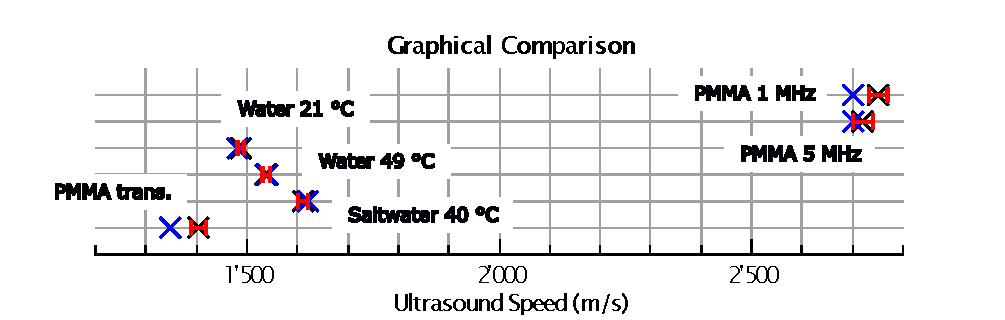
\includegraphics[scale=0.94]{results_ultrasound_speed}
	\caption{Graphical comparison between the calculated values (black cross with red uncertainty bar) and their respective literature values (blue cross). Especially the ultrasound speed of water is extremely close to the litearature value. The calculated sound velocities in PMMA at an oscillation frequency of 1 MHz are off by quite a bit (both logitudinal and transversal).}
	\label{fig:results_ultrasound_speed}
\end{figure}

\begin{figure}[H]
	\centering
	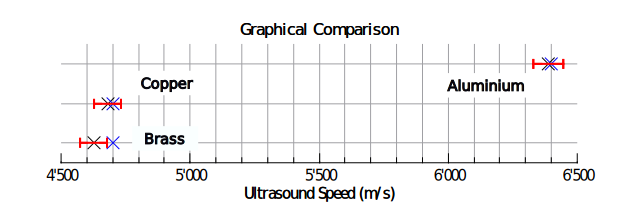
\includegraphics[scale=0.94]{results_metals}
	\caption{Graphical comparison of the three different metals aluminium, copper and brass. They are compared separately because their sound velocity is in a different range. This would have stretched out figure \ref{fig:results_ultrasound_speed} above and thus would have made it less readable. The literature values of the sound velocity (blue) in aluminium and copper lie inside the error bars of the respective metals.}
	\label{fig:results_metals}
\end{figure}

Table \ref{tab:Ultrasound_Speed} shows all calculated sound velocities and their respective literature values in one table.

\begin{table}[H]
	\centering
	\renewcommand{\arraystretch}{1.1}
	\begin{tabular}{|l|c|c|c|}
		\cline{2-4}
		\multicolumn{1}{c|}{} & $\boldsymbol{c}$ \textbf{@ 1 MHz} & $\boldsymbol{c}$ \textbf{@ 5 MHz} & \textbf{Litearture} \\
		\multicolumn{1}{c|}{} & in m/s & in m/s & in m/s \\
		\hline
		\textbf{PMMA} & $(2751\pm 19)$ & $(2721\pm 21)$ & $\approx 2700$ \\
		\hline
		\textbf{Aluminium} & - & $(6387\pm 59)$ & $\approx 6400$ \\
		\hline
		\textbf{Copper} & - & $(4680\pm 53)$ & $\approx 4700$ \\
		\hline
		\textbf{Brass} & - & $(4627\pm 52)$ & $\approx 4700$ \\
		\hline
		\textbf{Water 21 \textdegree C} & - & $(1488\pm 7)$ & $\approx 1483$ \\
		\hline
		\textbf{Water 49 \textdegree C} & - & $(1538\pm 8)$ & $\approx 1540$ \\
		\hline
		\textbf{Saltwater 40 \textdegree C} & - & $(1612\pm 10)$ & $\approx 1620$ \\
		\hline
		\textbf{PMMA trans.} & $(1405\pm 15)$ & - & $\approx 1350$ \\
		\hline
	\end{tabular}
	\caption{Summary of all calculated sound velocities and their respective literature values for the oscillation frequencies 1 MHz and 5 MHz.}
	\label{tab:Ultrasound_Speed}
\end{table}

% -----------------------------------------------------------------------------------------
\subsection{Attenuation Coefficient $\mu$}
\label{subsec:Attenuation_Coefficient}
The following figure \ref{fig:results_absorption} shows a graphical comparison between the two calculated attenuation coefficients and their uncertainties.

\begin{figure}[H]
	\centering
	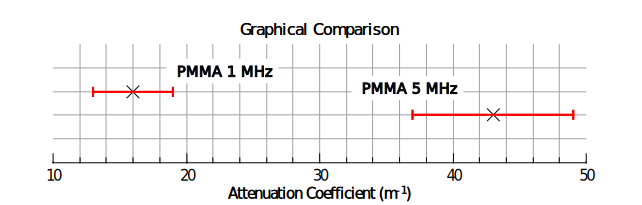
\includegraphics[scale=0.94]{results_absorption}
	\caption{Graphical comparison between the calculated values (black cross with red uncertainty bar) and their respective literature values (blue cross). The calculated attenuatin coefficient for PMMA at a frequency of 5 MHz is very imprecise. This is due to the fact, that the amplitude values are approaching 0 very fast. Thus, it is hard to get accurate readings (see figure \ref{fig:measuring_procedure}).}
	\label{fig:results_absorption}
\end{figure}

Table \ref{tab:Attenuation_Coefficient} shows the values of the calculated attenuation coefficients.

\begin{table}[H]
	\centering
	\renewcommand{\arraystretch}{1.1}
	\begin{tabular}{|l|c|c|}
		\cline{2-3}
		\multicolumn{1}{c|}{} & $\boldsymbol{\mu}$ \textbf{@ 1 MHz} & $\boldsymbol{\mu}$ \textbf{@ 5 MHz} \\
		\multicolumn{1}{c|}{} & in m$^{-1}$ & in m$^{-1}$ \\
		\hline
		\textbf{PMMA} & $(16\pm 3)$ & $(43\pm 6)$ \\
		\hline
	\end{tabular}
	\caption{Summary of the calculated attenuation coefficients for the oscillation frequencies 1 MHz and 5 MHz.}
	\label{tab:Attenuation_Coefficient}
\end{table}


% Bibliography
\printbibliography[heading=bibintoc]
\label{sec:literature}

% Glossary
\printglossaries

% Appendix
\begin{appendix}
	\section{Measurements}
	\label{sec:Measurements}
	\begin{table}[H]
		\centering
		\begin{tabular}{c|c|c}
			Order $m$ & Absolute Pos. 40 $\mu$m (mm) & Absolute Pos. 100 $\mu$m (mm) \\
			\hline\hline
			0 & 347.5 & 348.5 \\ \hline
			1 & 391.5 & 364.0 \\ \hline
			2 & 421.5 & 375.0 \\ \hline
			3 & 452.0 & 385.5 \\ \hline
			4 & 483.5 & 397.0 \\ \hline
			5 & 514.5 & 407.5 \\ \hline
			6 & 545.5 & 418.0 \\ \hline
			7 & 577.5 & 429.0 \\ \hline
			8 & 608.5 & 440.0 \\ \hline
			9 & - & 450.5 \\ \hline
			10 & - & 461.0 \\ \hline
		\end{tabular}
		\caption{Slit Apertures (maxima)\\x-value 40 $\mu$m = 1886 mm\\ x-value 100 $\mu$m = 1713 mm}
		\label{tab:Slit_Measurements}
	\end{table}

	\begin{table}[H]
		\centering
		\begin{tabular}{c|c|c}
			Order $m$ & Absolute Pos. 230 $\mu$m (mm) & Absolute Pos. 124 $\mu$m (mm) \\
			\hline\hline
			0 & 347.5 & 347.5 \\ \hline
			1 & 343.5 & 366.0 \\ \hline
			2 & 337.5 & 379.0 \\ \hline
			3 & 331.0 & 392.0 \\ \hline
			4 & 324.5 & 404.0 \\ \hline
			5 & 318.0 & 416.5 \\ \hline
			6 & 311.5 & 429.0 \\ \hline
			7 & 305.5 & 442.0 \\ \hline
			8 & 298.5 & 454.5 \\ \hline
			9 & 292.0 & 467.0 \\ \hline
			10 & 286.0 & 480.0 \\ \hline
			11 & 279.0 & 492.0 \\ \hline
			12 & 272.5 & 505.0 \\ \hline
			13 & 266.0 & 517.5 \\ \hline
			14 & 259.5 & - \\ \hline
			15 & 253.0 & - \\ \hline
			16 & 246.5 & - \\ \hline
			17 & 240.0 & - \\ \hline
			18 & 233.5 & - \\ \hline
		\end{tabular}
		\caption{Anti-Slit Apertures (maxima)\\x-value 230 $\mu$m = 2450 mm\\ x-value 124 $\mu$m = 2450 mm}
		\label{tab:Anti-Slit_Measurements}
	\end{table}

	\begin{table}[H]
		\centering
		\begin{tabular}{c|c|c}
			Bessel Coeff. $c_k$ & Absolute Pos. 150 $\mu$m (mm) & Absolute Pos. 100 $\mu$m (mm) \\
			\hline\hline
			0 & 348.0 & 347.0 \\ \hline
			1.220 & 356.0 & 359.0 \\ \hline
			2.233 & 363.0 & 369.5 \\ \hline
			3.238 & 370.0 & 380.0 \\ \hline
			4.241 & 377.0 & 390.5 \\ \hline
			5.243 & 384.0 & 401.0 \\ \hline
		\end{tabular}
		\caption{Circular Apertures (minima)\\x-value 150 $\mu$m = 1625 mm\\ x-value 100 $\mu$m = 1636 mm}
		\label{tab:Circular_Apertures_Measurements}
	\end{table}

	\begin{table}[H]
		\centering
		\begin{tabular}{c|c|c}
			Order $m$ & Absolute Pos. 28 $\mu$m (mm) & Absolute Pos. 50 $\mu$m (mm) \\
			\hline\hline
			0 & 348.0 & 347.5 \\ \hline
			1 & 294.0 & 280.5 \\ \hline
			2 & 259.0 & 254.0 \\ \hline
			3 & 220.0 & 227.5 \\ \hline
			4 & 185.0 & 200.5 \\ \hline
			5 & - & 173.5 \\ \hline
			6 & - & 147.0 \\ \hline
			7 & - & 120.0 \\ \hline
			8 & - & 92.5 \\ \hline
		\end{tabular}
		\caption{Cross-Grid Apertures (maxima)\\x-value 28 $\mu$m = 1639 mm\\ x-value 50 $\mu$m = 2112 mm}
		\label{tab:Cross-Grid_Measurements}
	\end{table}

	\newpage
	
	\section{MATLAB Angle Calculation}
	\label{sec:MATLAB_Angle_Calculation}
	\lstinputlisting{appendix/MATLAB.m}
	
	\newpage
	
	\section{MATLAB Error Calculation}
	\label{sec:MATLAB_Error_Calculation}
	\lstinputlisting{appendix/Error_Calculation.m}
\end{appendix}


% Debug
\ifdraft{
	\newpage
	\listoftodos[\section{To-Do}]
	\clearpage
}
{
}

\end{document}
